%%
%  ******************************************************************************
%  * #file    Szablon_raportu_EN_Latex.tex
%  * #author  Adrian Wójcik   adrian.wojcik(at)put.poznan.pl
%  *          
%  * #commit  Patryk Kościk   koscikpatryk(at)gmail.com
%  *          Modified the template for Projekt przejsciowy purposes          
%  *          
%  * #version 1.0
%  * #date    09-Mar-2022
%  * #brief   PROJPRZEJ
%  *
%  ******************************************************************************
%%  
\documentclass[11pt, a4paper]{article}

\usepackage{SM_template}

% Wypełnijcie te dyrektywy zgodnie z waszym tematem
% \lab      -> NAZWA CZUJNIKA, np.: 'DHT22'
% \comment  -> Króciutki opis co to, np.: 'Cyfrowy budżetowy czujnik temperatury'
%
\lab{Moduł W25Q64FV}
\comment{Moduł pamięci Serial Flash o pojemności 64 Mbit}

% Absolutny zakaz dotykania tego tutaj bo jak dotkiecie to coś jebnie
\university{Politechnika Poznańska}
\faculty{Wydział Automatyki, Robotyki i Elektrotechniki}
\institute{Instytut Robotyki i Inteligencji Maszynowej}
\department{Zakład Sterowania i Elektroniki Przemysłowej}
\addbibresource{bib/Flash.bib}
\nocite{*}


%%
%
% Początek dokumentu
%
%%
% \vspace{0.3cm}
% \begin{figure}[H]
% \centering
% \includegraphics[width=.7\linewidth]{fig/Flash/zasada_dzialania/zasada_dzialania.png}
% \caption{}
% \label{fig:sub3}
% \end{figure}
% \vspace{0.3cm}

% \begin{figure}[H]
% \centering
% \begin{subfigure}{.5\textwidth}
%   \centering
%   \includegraphics[width=.8\linewidth]{fig/Flash/zdj_modułu/widok_z_gory_bok.jpg}
%   \label{fig:sub1}
%   \caption{Zdjęcie modułu Flash}
% \end{subfigure}%
% \begin{subfigure}{.5\textwidth}
%   \centering
%   \includegraphics[width=.8\linewidth]{fig/Flash/zasada_dzialania/piezoelectric_inverse_effect.png}
%   \label{fig:sub2}
%   \caption{Odwrotny efekt piezoelektryczny}
% \end{subfigure}
% %\caption{Połączenie elektryczne}
% \label{fig:test}
% \end{figure}
\begin{document}

%% Strona tytułowa %%
\mainpage{{Flash/zdj_modułu/tytulowa.jpg}}
\newpage

\section{Opis elementu} \addcontentsline{toc}{section}{Wstęp}
%WP na low - pamięć ignoruje jakiekolwiek write/erase, dlatego jest podciągnięte pod vcc
%HOLD low jak CS jest low i wtedy clk i DI są ignorowane, bo i tak nie jest wybrany, hold jest po to, że jak parę urządzeń korzysta z jednej pamięci to żeby się nie okazało, że jedno urządzenie coś zapisuje, a drugie mu to usuwa/nadpisuje czymś innym
Głównym elementem opisywanego modułu jest pamięć Serial Flash W25Q64FV. Jest to pamięć typu NOR, o pojemności 64 Mbit, obsługiwana za pomocą interfejsu komunikacyjnego SPI. Pamięć flash dzieli się na dwa główne typy, w zależności od struktury komórek pamięci - NOR i NAND. Wykorzystywana w opisywanym module pamięć NOR charakteryzuje się jednoczesnym dostępem do wszystkich komórek pamięci, co powoduje że jej odczyt jest szybszy od tego w NAND, natomiast zapis lub usuwanie jej zawartości jest wolniejsze. Pamięć typu NOR potrzebuje także więcej mocy, w celu uruchomienia, ale podczas dalszych czynności pobiera jej mniej niż odpowiednik NAND.
\vspace{0.3cm}
\begin{figure}[H]
\centering
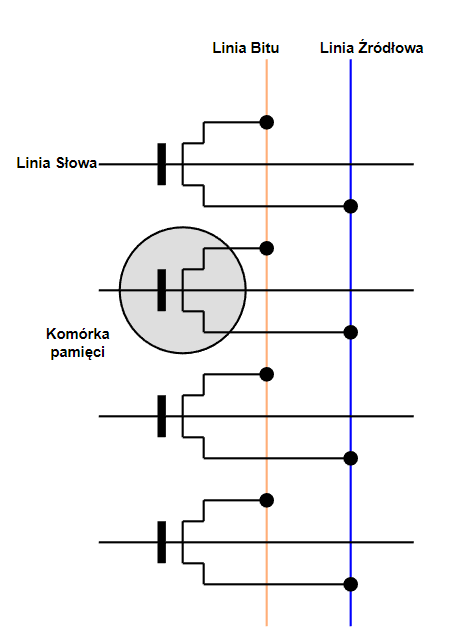
\includegraphics[width=.5\linewidth]{fig/Flash/zdj_modułu/NOR.PNG}
\caption{Schemat połączeń komórek pamięci w architekturze NOR}
\label{fig:sub3}
\end{figure}
\vspace{0.3cm}
Pamięć W25Q64FV jest pamięcią typu Flash SPI, która jest podzielona na strony (po 256B), sektory (4kB) i bloki (64 kB). Oznacza to, że pamięć 64 Mbit (8B) składa się z odpowiednio 128 bloków, każdy z nich z 16 sektorów, mających po 16 stron. %Istnieje także możliwość skorzystania z interfejsu QSPI do obsługi pamięci flash, który zamiast dwóch linii przesyłania danych, standardowych dla SPI (MISO i MOSI), wykorzystuje 4 linie. W przypadku microchipa W25Q64FV wykorzystuje się w tym celu dodatkowo piny HOLD i WP (ich cel został wyjaśniony w punkcie 1.1), jednak w opisywanym module są one zwarte z zasilaniem, więc nie można skorzystać z tej opcji.
\subsection{Opis modułu}
Moduł z pamięcią Flash W25Q64, oprócz samej pamięci, składa się z rezystora, diody LED (sygnalizującym o zasilaniu modułu), kondensatora i zestawu pinów. Microchip z pamięcią posiada 8 wejść:
\begin{itemize}
    \item CS - chip select - pin wykorzystywany w interfejsie SPI do wyboru odpowiedniego układu peryferyjnego,
    \item DO - data output - pin odczytu danych,
    \item WP - write protect - w przypadku podania stanu niskiego na ten pin blokowana jest możliwość wpisania lub usunięcia jakichkolwiek danych, w przypadku opisywanego modułu pin ten jest zwarty z zasilaniem,
    \item GND - masa,
    \item Vcc - zasilanie,
    \item HOLD - pin używany w przypadku gdy z danego microchipu pamięci korzysta pare urządzeń zewnętrznych, w celu zapobiegnięcia sytuacji, w której dane wykorzystywane przez jedno z urządzeń zostaną nadpisane przez inne, podanie na HOLD stanu niskiego spowoduje, że sygnał CLK i sygnały z pinu DI są ignorowane, w przypadku opisywanego modułu pin ten jest zwarty z zasilaniem,
    \item CLK - sygnał zegarowy (taktujący),
    \item DI - data input - pin wprowadzania danych.
\end{itemize}
\vspace{0.3cm}
\begin{figure}[H]
\centering
\begin{subfigure}{.5\textwidth}
  \centering
  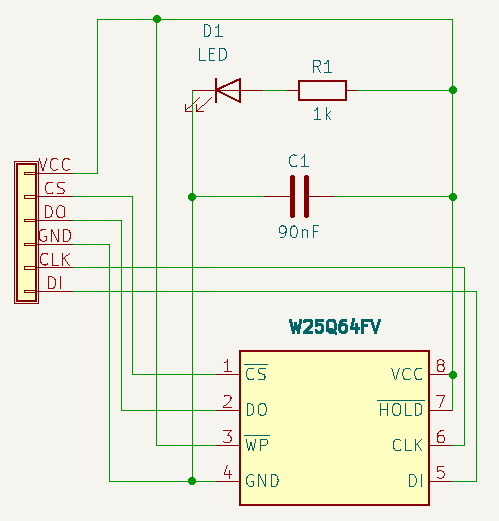
\includegraphics[width=.9\linewidth]{fig/Flash/zdj_modułu/schemat.PNG}
  \label{fig:sub1}
  \caption{Schemat elektryczny modułu z pamięcią Flash W25Q64}
\end{subfigure}%
\begin{subfigure}{.5\textwidth}
  \centering
  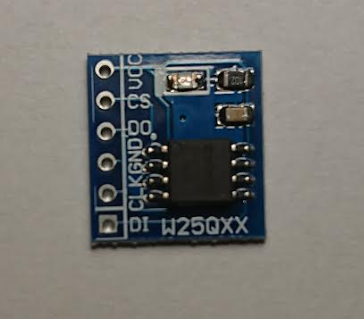
\includegraphics[width=.8\linewidth]{fig/Flash/zdj_modułu/zdjecie.PNG}
  \label{fig:sub2}
  \caption{Zdjęcie modułu}
\end{subfigure}
%\caption{Połączenie elektryczne}
\label{fig:test}
\end{figure}
\vspace{0.3cm}
\subsection{Zastosowania}
Moduły z pamięcią Flash można wykorzystać w projektach mikroprocesorowych wymagających większej ilości pamięci, niż udostępnia nam mikrokontroler (np. w przypadku ładowania grafik na wyświetlacz). Pamięć typowo o strukturze NOR jest wykorzystywana w urządzeniach wymagających niezawodności w zapisie małej ilości danych, takich jak telefony komórkowe, przyrządy laboratoryjno-pomiarowe lub urządzenia medyczne.


\newpage
\hypersetup{
    colorlinks=true,
    linkcolor=blue,
    filecolor=magenta,      
    urlcolor=cyan,
    pdftitle={Overleaf Example},
    pdfpagemode=FullScreen,
    }
\section{Użycie czujnika}
W celu zaprezentowania działania modułu wykorzystano mikrokontroler STM32 z wgranym odpowiednim programem. Została także przeprowadzona odpowiednia konfiguracja interfejsu SPI przy pomocy środowiska CubeIDE.
\vspace{0.3cm}
\begin{figure}[H]
\centering
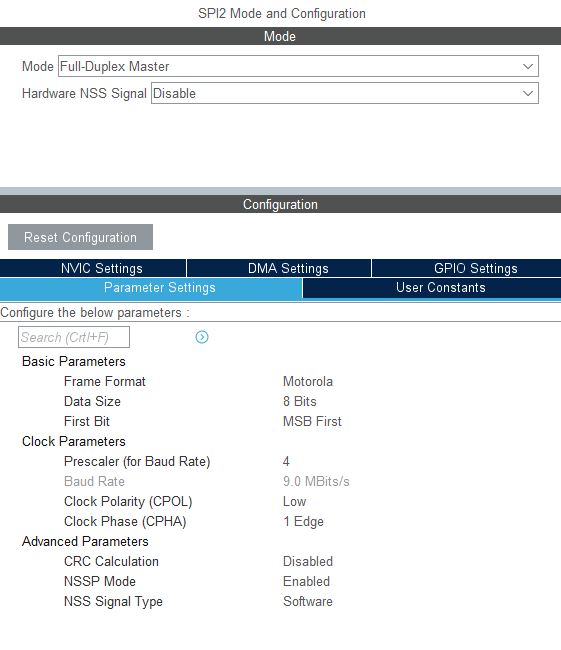
\includegraphics[width=.7\linewidth]{fig/Flash/działanie_ukladu/ICO.PNG}
\caption{Konfiguracja interfejsu SPI, wykorzystano następujące piny: MOSI - PC3, MISO - PC2, CLK - PB10, CS - skorzystano z GPIO na pinie PB0 w celu wysyłania sygnału, co pokazano na kolejnym obrazku}
\label{fig:sub3}
\end{figure}
\vspace{0.3cm}
\vspace{0.3cm}
\begin{figure}[H]
\centering
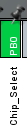
\includegraphics[width=.05\linewidth]{fig/Flash/działanie_ukladu/PB0.PNG}
\caption{Pin PB0 jako GPIO, nadano mu nazwę Chip\_Select}
\label{fig:sub3}
\end{figure}
\vspace{0.3cm}
\vspace{0.3cm}
\begin{figure}[H]
\centering
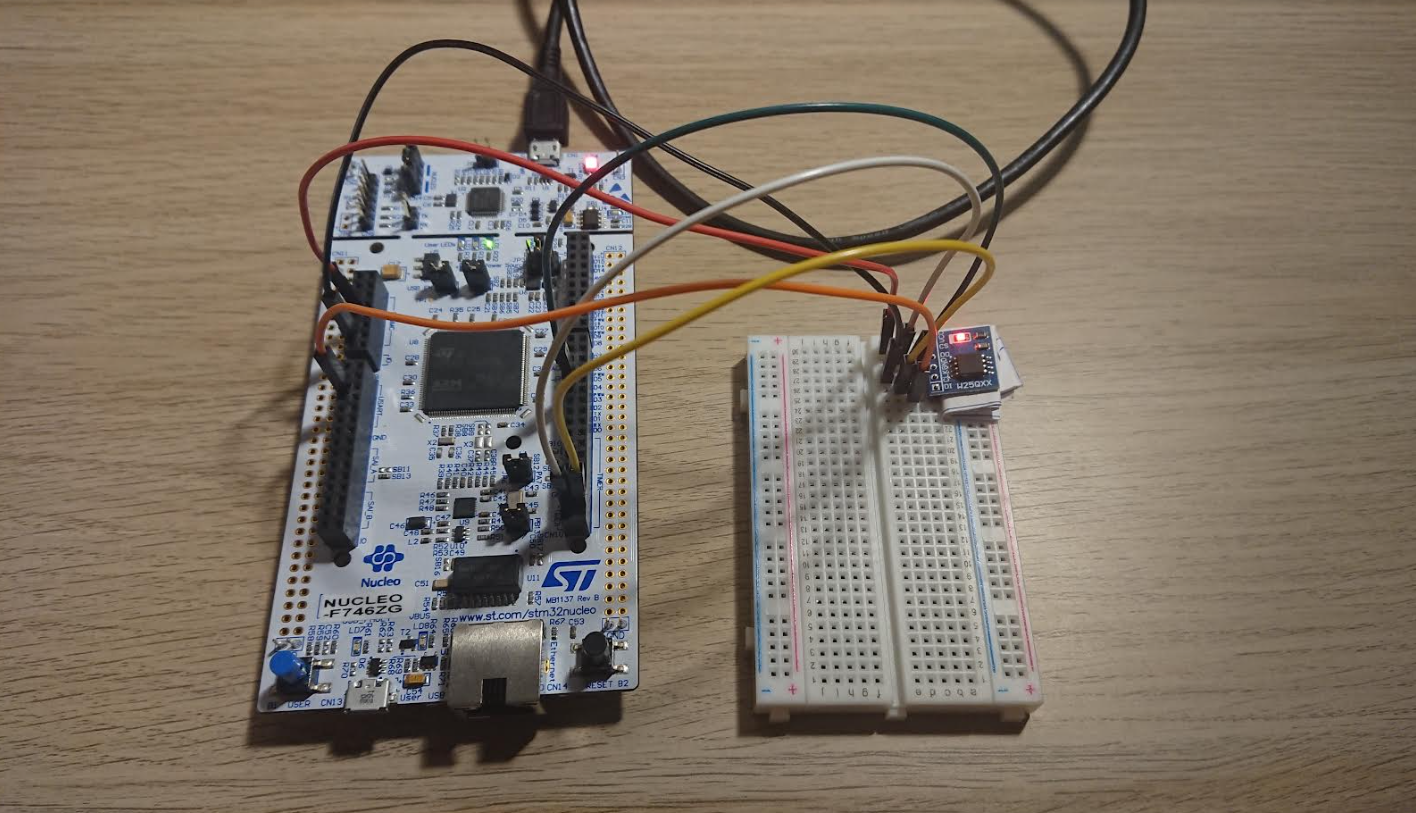
\includegraphics[width=.9\linewidth]{fig/Flash/działanie_ukladu/polaczenia.PNG}
\caption{Połączona pamięć flash z mikrokontrolerem}
\label{fig:sub3}
\end{figure}
\vspace{0.3cm}
Aby zaprezentować podstawową funkcjonalność pamięci skorzystano z gotowej biblioteki zewnętrznej, która umożliwia odpowiednie zapisywanie i odczytywanie adresów w pamięci. Program najpierw odczytywał 256 wartości od określonego adresu, następnie nadpisywał je wartościami od 0 do 255 i ponownie odczytywał. 
\vspace{0.3cm}
\begin{figure}[H]
\centering
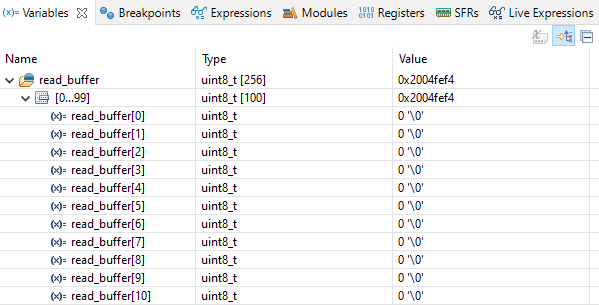
\includegraphics[width=.9\linewidth]{fig/Flash/działanie_ukladu/read_0.PNG}
\caption{Początkowe wartości bufora sczytującego}
\label{fig:sub3}
\end{figure}
\vspace{0.3cm}
\vspace{0.3cm}
\begin{figure}[H]
\centering
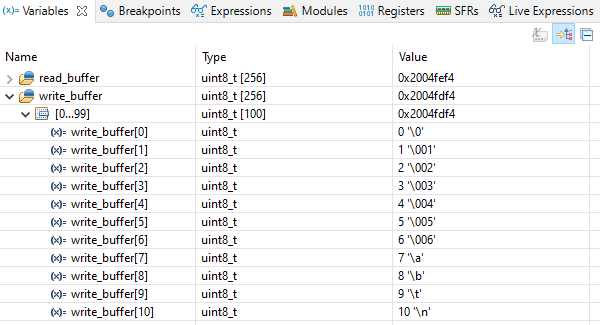
\includegraphics[width=.9\linewidth]{fig/Flash/działanie_ukladu/write.PNG}
\caption{Wartości bufora wpisującego wartości}
\label{fig:sub3}
\end{figure}
\vspace{0.3cm}
\vspace{0.3cm}
\begin{figure}[H]
\centering
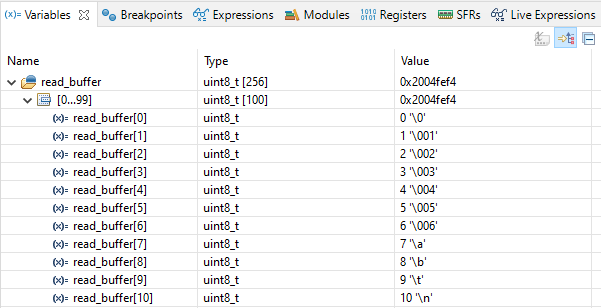
\includegraphics[width=.9\linewidth]{fig/Flash/działanie_ukladu/read_255.PNG}
\caption{Wartości bufora sczytującego po odczytaniu wartości zapisanych}
\label{fig:sub3}
\end{figure}
\vspace{0.3cm}



%\printbibliography[heading=bibintoc]

\end{document}